% Presentation for MA 232 Group Project 2. Build: latexmk -xelatex slides.tex
% Speaker notes: latexmk -xelatex -jobname=slides_notes slides.tex  (see Makefile)
\documentclass[aspectratio=169,11pt]{beamer}
\usepackage{fontspec}
\setsansfont{Inter}[Scale=0.95]
\usepackage{amsmath}
\usepackage{unicode-math}
\setmathfont{Latin Modern Math}
\setmathfont{Inter}[range={up/num,up/Latin,up/latin}, Scale=0.95]
\usepackage{booktabs}
\usefonttheme{professionalfonts}
\graphicspath{{../figures/}}
% Generated by scripts/run_analysis.py. Do not edit by hand.
% Use numeric macros inside math mode so minus signs render correctly.
\newcommand{\alphaA}{63}
\newcommand{\alphaB}{71}
\newcommand{\alphaC}{67}
\newcommand{\betaA}{39}
\newcommand{\betaB}{31}
\newcommand{\betaC}{35}
\newcommand{\crihiA}{0.709}
\newcommand{\crihiB}{0.781}
\newcommand{\crihiC}{0.745}
\newcommand{\criloA}{0.522}
\newcommand{\criloB}{0.604}
\newcommand{\criloC}{0.562}
\newcommand{\cseBA}{0.0668}
\newcommand{\cseBC}{0.0659}
\newcommand{\cseCA}{0.0678}
\newcommand{\cwaldhiBA}{0.211}
\newcommand{\cwaldhiBC}{0.169}
\newcommand{\cwaldhiCA}{0.173}
\newcommand{\cwaldloBA}{-0.051}
\newcommand{\cwaldloBC}{-0.089}
\newcommand{\cwaldloCA}{-0.093}
\newcommand{\dhiBA}{0.207}
\newcommand{\dhiBC}{0.167}
\newcommand{\dhiCA}{0.170}
\newcommand{\dloBA}{-0.051}
\newcommand{\dloBC}{-0.089}
\newcommand{\dloCA}{-0.092}
\newcommand{\dmeanBA}{0.078}
\newcommand{\dmeanBC}{0.039}
\newcommand{\dmeanCA}{0.039}
\newcommand{\dsdBA}{0.066}
\newcommand{\dsdBC}{0.065}
\newcommand{\dsdCA}{0.067}
\newcommand{\elossA}{0.0913}
\newcommand{\elossB}{0.0128}
\newcommand{\elossC}{0.0521}
\newcommand{\elossptsA}{9.13}
\newcommand{\elossptsB}{1.28}
\newcommand{\elossptsC}{5.21}
\newcommand{\emax}{0.7089}
\newcommand{\mcdraws}{2{,}000{,}000}
\newcommand{\mcmaxabsz}{0.71}
\newcommand{\mcpbestB}{0.6807}
\newcommand{\mcpgtBA}{0.8823}
\newcommand{\mcseBA}{0.00023}
\newcommand{\mcsebestB}{0.00033}
\newcommand{\mcseed}{20261008}
\newcommand{\mczBA}{-0.71}
\newcommand{\mczbestB}{0.54}
\newcommand{\meanA}{0.6176}
\newcommand{\meanB}{0.6961}
\newcommand{\meanC}{0.6569}
\newcommand{\meanfracA}{\tfrac{63}{102}}
\newcommand{\meanfracB}{\tfrac{71}{102}}
\newcommand{\meanfracC}{\tfrac{67}{102}}
\newcommand{\medianA}{0.6184}
\newcommand{\medianB}{0.6974}
\newcommand{\medianC}{0.6579}
\newcommand{\mleA}{0.62}
\newcommand{\mleB}{0.70}
\newcommand{\mleC}{0.66}
\newcommand{\mmeanexA}{0.617647}
\newcommand{\mmeanexB}{0.696078}
\newcommand{\mmeanexC}{0.656863}
\newcommand{\mmeanliA}{0.617600}
\newcommand{\mmeanliB}{0.696000}
\newcommand{\mmeanliC}{0.656800}
\newcommand{\mmeanlierrA}{-4.7\times 10^{-5}}
\newcommand{\mmeanlierrB}{-7.8\times 10^{-5}}
\newcommand{\mmeanlierrC}{-6.3\times 10^{-5}}
\newcommand{\mmeantkA}{0.617595}
\newcommand{\mmeantkB}{0.696016}
\newcommand{\mmeantkC}{0.656805}
\newcommand{\mmeantkerrA}{-5.2\times 10^{-5}}
\newcommand{\mmeantkerrB}{-6.2\times 10^{-5}}
\newcommand{\mmeantkerrC}{-5.7\times 10^{-5}}
\newcommand{\moddsexA}{1.657895}
\newcommand{\moddsexB}{2.366667}
\newcommand{\moddsexC}{1.970588}
\newcommand{\moddsliA}{1.657895}
\newcommand{\moddsliB}{2.366667}
\newcommand{\moddsliC}{1.970588}
\newcommand{\moddslierrA}{0}
\newcommand{\moddslierrB}{0}
\newcommand{\moddslierrC}{0}
\newcommand{\moddstkA}{1.657832}
\newcommand{\moddstkB}{2.366480}
\newcommand{\moddstkC}{1.970479}
\newcommand{\moddstkerrA}{-6.3\times 10^{-5}}
\newcommand{\moddstkerrB}{-1.9\times 10^{-4}}
\newcommand{\moddstkerrC}{-1.1\times 10^{-4}}
\newcommand{\modeA}{0.6200}
\newcommand{\modeB}{0.7000}
\newcommand{\modeC}{0.6600}
\newcommand{\onempBA}{0.884}
\newcommand{\onempBC}{0.728}
\newcommand{\onempCA}{0.722}
\newcommand{\pbestA}{0.071}
\newcommand{\pbestB}{0.681}
\newcommand{\pbestC}{0.248}
\newcommand{\pbestlongA}{0.071201793908}
\newcommand{\pbestlongB}{0.680515173383}
\newcommand{\pbestlongC}{0.248283032709}
\newcommand{\pgtBA}{0.882}
\newcommand{\pgtBC}{0.726}
\newcommand{\pgtCA}{0.721}
\newcommand{\pgtlongBA}{0.882419268177}
\newcommand{\pgtlongBC}{0.726473157011}
\newcommand{\pgtlongCA}{0.720933436473}
\newcommand{\pmarginBA}{0.667}
\newcommand{\pmarginBC}{0.435}
\newcommand{\pmarginCA}{0.437}
\newcommand{\predcovA}{0.961}
\newcommand{\predcovB}{0.965}
\newcommand{\predcovC}{0.958}
\newcommand{\predhiA}{75}
\newcommand{\predhiB}{82}
\newcommand{\predhiC}{78}
\newcommand{\predloA}{48}
\newcommand{\predloB}{56}
\newcommand{\predloC}{52}
\newcommand{\predmeanA}{61.8}
\newcommand{\predmeanB}{69.6}
\newcommand{\predmeanC}{65.7}
\newcommand{\predsdA}{6.8}
\newcommand{\predsdB}{6.4}
\newcommand{\predsdC}{6.6}
\newcommand{\pvalBA}{0.116}
\newcommand{\pvalBC}{0.272}
\newcommand{\pvalCA}{0.278}
\newcommand{\sBtendec}{B}
\newcommand{\sBtenelossB}{0.0135}
\newcommand{\sBtenmeanB}{0.667}
\newcommand{\sBtenpBA}{0.859}
\newcommand{\sBtenpBC}{0.707}
\newcommand{\sBtenpbestA}{0.086}
\newcommand{\sBtenpbestB}{0.652}
\newcommand{\sBtenpbestC}{0.262}
\newcommand{\sBttdec}{B}
\newcommand{\sBttelossB}{0.0129}
\newcommand{\sBttmeanB}{0.692}
\newcommand{\sBttpBA}{0.880}
\newcommand{\sBttpBC}{0.724}
\newcommand{\sBttpbestA}{0.073}
\newcommand{\sBttpbestB}{0.677}
\newcommand{\sBttpbestC}{0.250}
\newcommand{\sJefdec}{B}
\newcommand{\sJefelossB}{0.0128}
\newcommand{\sJefmeanB}{0.698}
\newcommand{\sJefpBA}{0.884}
\newcommand{\sJefpBC}{0.728}
\newcommand{\sJefpbestA}{0.070}
\newcommand{\sJefpbestB}{0.682}
\newcommand{\sJefpbestC}{0.247}
\newcommand{\sUnidec}{B}
\newcommand{\sUnielossB}{0.0128}
\newcommand{\sUnimeanB}{0.696}
\newcommand{\sUnipBA}{0.882}
\newcommand{\sUnipBC}{0.726}
\newcommand{\sUnipbestA}{0.071}
\newcommand{\sUnipbestB}{0.681}
\newcommand{\sUnipbestC}{0.248}
\newcommand{\scenapBA}{0.882}
\newcommand{\scenapBC}{0.726}
\newcommand{\scenapbest}{0.681}
\newcommand{\scenbpBA}{0.954}
\newcommand{\scenbpBC}{0.804}
\newcommand{\scenbpbest}{0.785}
\newcommand{\scencpBA}{0.981}
\newcommand{\scencpBC}{0.853}
\newcommand{\scencpbest}{0.845}
\newcommand{\scencross}{750}
\newcommand{\scendpBA}{0.996}
\newcommand{\scendpBC}{0.912}
\newcommand{\scendpbest}{0.911}
\newcommand{\scenepBA}{{>}\,0.999}
\newcommand{\scenepBC}{0.972}
\newcommand{\scenepbest}{0.972}
\newcommand{\sdA}{0.0479}
\newcommand{\sdB}{0.0453}
\newcommand{\sdC}{0.0468}
\newcommand{\shrinkw}{0.980}
\newcommand{\waldhiA}{0.715}
\newcommand{\waldhiB}{0.790}
\newcommand{\waldhiC}{0.753}
\newcommand{\waldloA}{0.525}
\newcommand{\waldloB}{0.610}
\newcommand{\waldloC}{0.567}
\newcommand{\waldseA}{0.0485}
\newcommand{\waldseB}{0.0458}
\newcommand{\waldseC}{0.0474}
\newcommand{\zpoolBA}{1.19}
\newcommand{\zpoolBC}{0.61}
\newcommand{\zpoolCA}{0.59}

% Group members. The report's title block and its PDF metadata both read this file.
\newcommand{\projectauthors}{%
  Aditya Singh (250003007) \quad Hiransh Anand (250041018) \quad Parth Pawar (250041030)\\
  Tirthanker Singh (250003081) \quad Gulam Abbas (250041016)}
\newcommand{\projectauthorsplain}{Aditya Singh, Hiransh Anand, Parth Pawar, Tirthanker Singh, Gulam Abbas}


\ifdefined\shownotes
  \setbeameroption{show only notes}
\fi

\definecolor{ink}{HTML}{0B0B0B}
\definecolor{ink2}{HTML}{52514E}
\definecolor{tA}{HTML}{2A78D6}
\definecolor{tB}{HTML}{EB6834}
\definecolor{tC}{HTML}{1BAF7A}
\setbeamercolor{normal text}{fg=ink,bg=white}
\setbeamercolor{frametitle}{fg=ink,bg=white}
\setbeamercolor{title}{fg=ink}
\setbeamercolor{structure}{fg=ink2}
\setbeamercolor{alerted text}{fg=tB}
\setbeamerfont{frametitle}{series=\bfseries,size=\Large}
\setbeamertemplate{navigation symbols}{}
\setbeamertemplate{itemize items}{\textendash}
\setbeamertemplate{footline}{\hfill\textcolor{ink2}{\scriptsize\insertframenumber/\inserttotalframenumber}\hspace{1.2em}\vspace{0.8em}}
\setbeamertemplate{note page}{\vspace{1em}\insertnote}

\newcommand{\BetaD}{\text{Beta}}
\newcommand{\headline}[1]{{\Huge\bfseries #1}}

\title{Which Treatment Should We Choose?}
\subtitle{A Bayesian comparison of three treatments}
\author{\projectauthors}
\hypersetup{pdfauthor={\projectauthors}}
\institute{MA 232 Bayesian Statistical Methods \textbullet{} Group Project 2}
\date{October 2026}

\begin{document}

\begin{frame}
\titlepage
\note{Our project compares three treatments from a small simulated trial and asks which one to use.
Everything we show comes from one script, and every probability is computed exactly.}
\end{frame}

\begin{frame}{The question}
\begin{columns}[T]
\column{0.45\textwidth}
\begin{tabular}{lrrr}
\toprule
 & Patients & Successes & Rate\\
\midrule
\textcolor{tA}{A} & 100 & 62 & $\mleA$\\
\textcolor{tB}{B} & 100 & 70 & $\mleB$\\
\textcolor{tC}{C} & 100 & 66 & $\mleC$\\
\bottomrule
\end{tabular}

\vspace{1em}
\textcolor{ink2}{\small Simulated clinical-trial data from the project sheet.}
\column{0.5\textwidth}
\begin{itemize}
\item How large is each success probability, and how sure are we?
\item How do the treatments differ?
\item What is $P(\text{B better than A})$?
\item What is $P(\text{B is the best})$?
\item Which treatment should we choose?
\end{itemize}
\end{columns}
\note{B has the highest raw success rate, 70 out of 100, but with only 100 patients each the gaps
of 4 and 8 percentage points could be noise. The question is how much the data really tell us.}
\end{frame}

\begin{frame}{Model: binomial data, Beta prior}
\begin{itemize}
\item Each patient succeeds independently with probability $\theta$:
$\;f(\mathbf{x}\mid\theta)=\theta^{s}(1-\theta)^{n-s}$
\item Neyman--Fisher: the count $s$ is sufficient; only the table matters
\item Uniform prior $\BetaD(1,1)$ gives the conjugate posterior $\BetaD(s+1,\,n-s+1)$
\end{itemize}
\vspace{0.6em}
\begin{center}
\Large
$\theta_A\sim\BetaD(\alphaA,\betaA)\qquad\theta_B\sim\BetaD(\alphaB,\betaB)\qquad\theta_C\sim\BetaD(\alphaC,\betaC)$
\end{center}
\vspace{0.4em}
\textcolor{ink2}{\small Module 3 (sufficiency, MLE) \textbullet{} Module 4, Example 4.6 (Beta--binomial)}
\note{The likelihood depends on the data only through the number of successes, so the table is all
we need. A uniform prior expresses no preference, and the posterior is again Beta: add successes to
the first parameter and failures to the second.}
\end{frame}

\begin{frame}{Estimates and uncertainty}
\begin{columns}[c]
\column{0.62\textwidth}
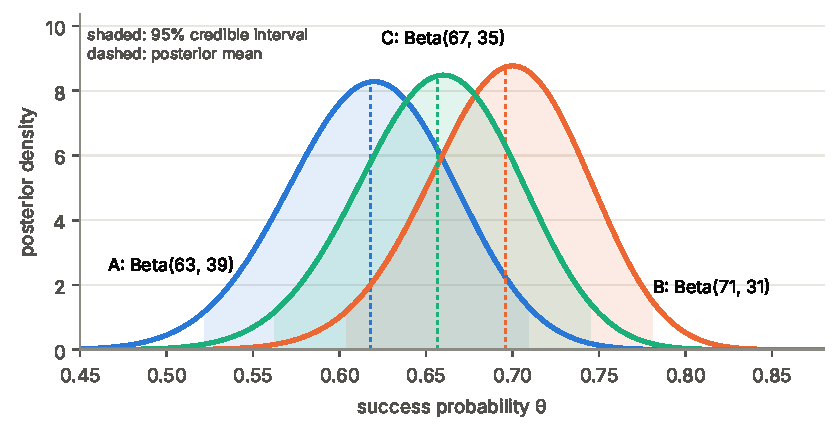
\includegraphics[width=\linewidth]{fig1_posteriors.pdf}
\column{0.36\textwidth}
\small
\begin{tabular}{lcc}
\toprule
 & Post.\ mean & 95\% CrI\\
\midrule
A & $\meanA$ & $\criloA$--$\crihiA$\\
B & $\meanB$ & $\criloB$--$\crihiB$\\
C & $\meanC$ & $\criloC$--$\crihiC$\\
\bottomrule
\end{tabular}

\vspace{0.8em}
Each rate is known to about $\pm9$ points.\\[0.3em]
Mean $<$ median $<$ mode: left-skewed posteriors.
\end{columns}
\note{The three posteriors overlap a lot. B is ahead with posterior mean \meanB, but its credible
interval overlaps both others. The posterior mean is the Bayes estimator under squared-error loss;
median and mode are in the report.}
\end{frame}

\begin{frame}{How do the treatments differ?}
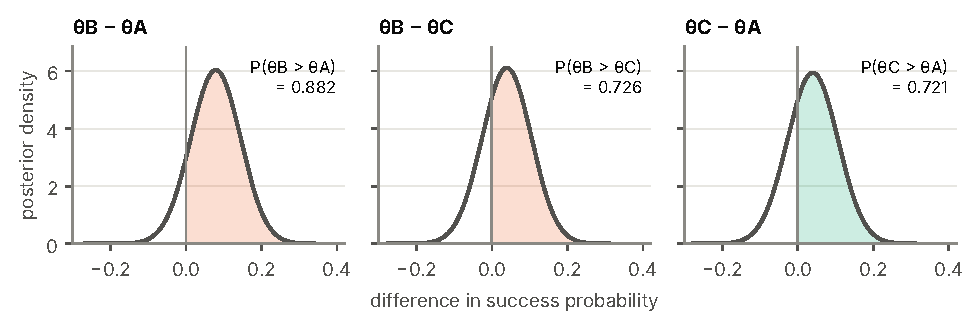
\includegraphics[width=\linewidth]{fig2_differences.pdf}
\vspace{0.2em}
\begin{columns}[T]
\column{0.5\textwidth}
\alert{$P(\theta_B>\theta_A\mid\text{data})=\pgtBA$}\\
\small$P(\theta_B-\theta_A>0.05)=\pmarginBA$
\column{0.48\textwidth}
\small Classical test of B vs A: $p=\pvalBA$, ``not significant''.\\
It cannot say how likely B is to be better.
\end{columns}
\note{The shaded area is the probability that the first treatment is better. B beats A with
probability \pgtBA, but a gain of more than 5 points is less certain, \pmarginBA. The p-value of
\pvalBA{} answers a different question.}
\end{frame}

\begin{frame}{Exact, not simulated}
\[
P(\theta_B>\theta_A\mid\text{data})=\int_0^1 f_B(t)\,F_A(t)\,dt
\]
\begin{itemize}
\item Whole-number Beta parameters: $f_B$ and $F_A$ are \textbf{polynomials} with rational coefficients
\item So the answer is an exact fraction: $\pgtlongBA\ldots$
\item Same fraction from an independent finite-sum formula; quadrature agrees to $10^{-12}$
\item Monte Carlo, $\mcdraws$ draws: every estimate within $\mcmaxabsz$ standard errors
\end{itemize}
\note{Because the parameters are whole numbers, the densities and CDFs are polynomials, so these
integrals have exact rational values. We checked them with a second exact formula, numerical
integration and simulation.}
\end{frame}

\begin{frame}{Which treatment is best?}
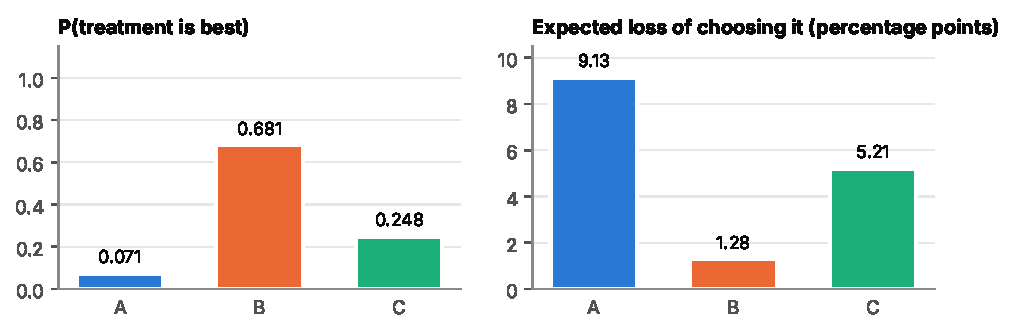
\includegraphics[width=\linewidth]{fig3_best.pdf}
\begin{center}
$P(k\text{ best})=\int_0^1 f_k(t)\prod_{j\neq k}F_j(t)\,dt$ \qquad
\alert{$P(\text{B best})=\pbestB$}
\end{center}
\note{B is the most likely best treatment, \pbestB, then C, \pbestC. On the right is the expected
loss of each choice, the success rate we would expect to give up by not picking the true best.}
\end{frame}

\begin{frame}{Choosing is a Bayes decision}
\begin{columns}[T]
\column{0.42\textwidth}
\textbf{Minimise posterior expected loss}\\[0.3em]
\small
Opportunity loss $\max_j\theta_j-\theta_k$\\ $\Rightarrow$ largest posterior mean: \alert{B}\\[0.4em]
Zero--one loss (not the best)\\ $\Rightarrow$ largest $P(\text{best})$: \alert{B}\\[0.6em]
\textcolor{ink2}{Module 4, Definition 4.3}
\column{0.56\textwidth}
\small
\begin{tabular}{lccc}
\toprule
Prior & $P(\theta_B>\theta_A)$ & $P(\text{B best})$ & Choice\\
\midrule
$\BetaD(1,1)$ & $\sUnipBA$ & $\sUnipbestB$ & \sUnidec\\
Jeffreys & $\sJefpBA$ & $\sJefpbestB$ & \sJefdec\\
$\BetaD(2,2)$ & $\sBttpBA$ & $\sBttpbestB$ & \sBttdec\\
$\BetaD(10,10)$ & $\sBtenpBA$ & $\sBtenpbestB$ & \sBtendec\\
\bottomrule
\end{tabular}
\end{columns}
\note{Both natural loss functions pick B, and the choice does not change under any of four priors,
including a fairly strong Beta(10,10) prior centred on 50 percent.}
\end{frame}

\begin{frame}{How sure are we about B over C?}
\begin{columns}[c]
\column{0.55\textwidth}
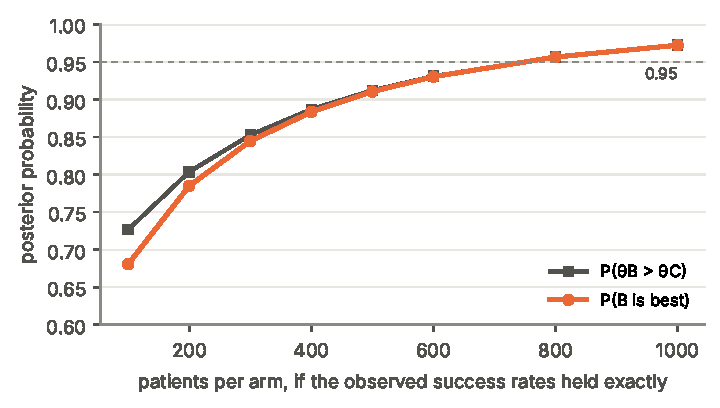
\includegraphics[width=\linewidth]{fig4_more_data.pdf}
\column{0.43\textwidth}
\begin{itemize}
\item $P(\theta_B>\theta_C)=\pgtBC$ only
\item 95\% CrI for $\theta_B-\theta_C$: $\dloBC$ to $\dhiBC$
\item If the rates held, $P(\text{B best})$ would reach $0.95$ at about $\scencross$ patients per arm
\end{itemize}
\textcolor{ink2}{\scriptsize Illustration only, not a prediction.}
\end{columns}
\note{B is clearly better than A, but only modestly ahead of C. Even if the observed rates held
exactly, we would need roughly \scencross{} patients per arm to be 95 percent sure B is best.}
\end{frame}

\begin{frame}{Course check: Lindley and Tierney--Kadane (Module 5)}
\small
\begin{tabular}{lccccc}
\toprule
 & Exact $E[\theta]$ & Lindley error & T--K error & Exact $E[\text{odds}]$ & T--K error\\
\midrule
A & $\mmeanexA$ & $\mmeanlierrA$ & $\mmeantkerrA$ & $\moddsexA$ & $\moddstkerrA$\\
B & $\mmeanexB$ & $\mmeanlierrB$ & $\mmeantkerrB$ & $\moddsexB$ & $\moddstkerrB$\\
C & $\mmeanexC$ & $\mmeanlierrC$ & $\mmeantkerrC$ & $\moddsexC$ & $\moddstkerrC$\\
\bottomrule
\end{tabular}
\normalsize
\begin{itemize}
\item Our code reproduces the slides' example: Lindley $1.9965$, T--K $1.995138$
\item Errors $\approx10^{-4}=O(n^{-2})$; Lindley is \emph{exact} for the odds, $(s+1)/(n-s)$
\end{itemize}
\note{Our problem has exact answers, so it is a clean test of the Module 5 approximations. After
reproducing the course example, both methods are accurate to about one part in ten thousand, and
Lindley's terms add up exactly for the odds.}
\end{frame}

\begin{frame}{Recommendation}
\begin{center}
\headline{Choose treatment \textcolor{tB}{B}}
\end{center}
\vspace{0.4em}
\begin{itemize}
\item Highest success rate: $\meanB$ (95\% CrI $\criloB$--$\crihiB$)
\item Most likely best: $\pbestB$; smallest expected loss: $\elossptsB$ points
\item The same under every prior we tried
\end{itemize}
\vspace{0.3em}
\textcolor{ink2}{\small Caveats: B vs C is not settled; simulated data; success is the only outcome;
independent arms assumed. A further B-versus-C trial is justified if the stakes are high.}
\note{Our recommendation is B. It has the highest estimated success rate, the highest chance of being
best and the smallest expected loss, under every prior. B versus C is the open question.}
\end{frame}

\end{document}
